%% Tri-Loop Adaptive Co-Design --- IEEE Trans. Sustainable Energy submission
%% Status: DRAFT v0.2 (2026-05-02) — restructured for tier-1 depth
%% Authors: D. N. Prakoso, A. Soeprijanto (corresponding), D. F. U. Putra, A. W. Wardhana, B. Winarno

\documentclass[journal]{IEEEtran}

\usepackage{amsmath,amssymb,amsfonts}
\usepackage{algorithmic}
\usepackage{graphicx}
\usepackage[utf8]{inputenc}
\usepackage{textcomp}
\usepackage{xcolor}
\usepackage{cite}
\usepackage{booktabs}
\usepackage{siunitx}
\usepackage{subcaption}
\usepackage{multirow}
\usepackage{enumitem}
\usepackage{url}
\usepackage{hyperref}
\hypersetup{colorlinks=true,linkcolor=blue,urlcolor=blue,citecolor=blue}

\graphicspath{{figures/}}

\begin{document}

\title{Tri-Loop Adaptive Co-Design of Virtual Inertia, Damping, and
Battery Storage Coordination for High-Penetration PV--BESS Systems
under Weak Tropical Grids}

\author{Dimas~Nur~Prakoso,
        Adi~Soeprijanto,~\IEEEmembership{Member,~IEEE,}
        Dimas~Fajar~Uman~Putra,
        Ananthyo~Whisnu~Wardhana,
        and~Basuki~Winarno%
\thanks{Manuscript submitted for review.}%
\thanks{D.~N.~Prakoso, A.~Soeprijanto, D.~F.~U.~Putra, and A.~W.~Wardhana are with the Department of Electrical Engineering, Institut Teknologi Sepuluh Nopember (ITS), Surabaya 60111, Indonesia (e-mail: 7022251005@student.its.ac.id; adisup@ee.its.ac.id; dimasfup@its.ac.id; 6022251032@student.its.ac.id).}%
\thanks{B.~Winarno is with Politeknik Negeri Madiun, Indonesia (e-mail: basuki@pnm.ac.id).}%
\thanks{Corresponding author: A.~Soeprijanto (e-mail: adisup@ee.its.ac.id).}%
\thanks{Source code, raw simulation data, and reproducibility manifest:\\\url{https://github.com/Power-Simulations/pemodelan-paper1}.}}


\markboth{IEEE Transactions on Sustainable Energy,~Vol.~XX, No.~X, May~2026}%
{Prakoso \MakeLowercase{\textit{et al.}}: Tri-Loop Adaptive Co-Design for PV--BESS Systems}

\maketitle

\begin{abstract}
Adaptive virtual-inertia control (VIC) for grid-connected
photovoltaic--battery-energy-storage (PV--BESS) systems has matured
along fuzzy-logic, hyperbolic-tangent, and learning-based strands.
This paper makes two contributions. \emph{First}, we identify a
previously underreported failure mode shared by all three strands: a
self-sustaining $\sim$5.7\,kW peak-to-peak limit cycle in the
active-power injection of a 125\,kW plant, fed by the closed-loop
interaction between the saturating gain, activation dead-band, and
BESS-supervisor switching state machine. The phenomenon is invisible
to linear small-signal analysis ($\zeta_{\min}=0.921$) yet imposes a
measurable energy-throughput penalty; a windowed FFT of the
steady-state injection isolates the switching-mode oscillation.
\emph{Second}, we propose a \emph{tri-loop adaptive co-design}: a
single supervisory layer that simultaneously schedules
smooth-saturating $H(\dot\omega)$ and $D(\Delta\omega)$, MPPT/VIC
mixing weight $\alpha(\Delta\omega,\dot\omega)$, and SOC- and
severity-aware BESS contribution share
$\beta(\Delta\omega,\dot\omega,\mathrm{SOC})$. The scheme suppresses
limit-cycle amplitude by $\sim$3 orders of magnitude while satisfying
IEEE~1547-2018 Category~I thresholds (RoCoF $\leq 0.5$\,Hz/s,
$|\Delta f|\leq 0.4$\,Hz) in 87\% of a 1\,000-sample Monte Carlo
sweep over SCR, system inertia, disturbance magnitude, initial SOC,
and gain perturbation; joint pass rate reaches 100\% at ENTSO-E
(1\,Hz/s) and Category~II (2\,Hz/s) thresholds. An off-equilibrium
small-signal analysis shows the dominant-mode time constant is
1.5--2.2$\times$ shorter than baselines once adaptive gains activate.
Five canonical disturbances plus a 24-h Madiun, Indonesia case driven
by NASA POWER MERRA-2 hourly irradiance for 2025 confirm the
conclusions. All code and data are released under MIT license.
\end{abstract}

\begin{IEEEkeywords}
Adaptive virtual inertia, battery energy storage, weak-grid frequency
stability, photovoltaic system, limit-cycle robustness.
\end{IEEEkeywords}

% =====================================================================
\section{Introduction}\label{sec:intro}
% =====================================================================
\IEEEPARstart{T}{he} accelerating displacement of synchronous
generation by inverter-based resources (IBRs) has eroded the inertial
reserve that legacy grids relied upon for frequency-event arrest
\cite{tielens2016relevance,milano2018foundations}. At inverter
penetration levels above 70\%, the rate-of-change-of-frequency
(RoCoF) following a generation-loss event routinely approaches or
exceeds the operating-envelope thresholds adopted by transmission
operators worldwide. IEEE~Std~1547-2018 \cite{ieee15472018} mandates
RoCoF ride-through at $0.5$\,Hz/s for Category~I devices, $2.0$\,Hz/s
for Category~II, and $3.0$\,Hz/s for Category~III---categories
chosen by the local Authority Governing Interconnection Requirements
(AGIR) according to the bulk-system reliability needs of the
interconnected grid. The transmission-level standard
IEEE~Std~2800-2022 \cite{ieee28002022} extends ride-through to up to
5\,Hz/s for high-voltage IBR plants; the European EN~50549-1
\cite{en505492019} and AEMO~Australia typically enforce 1--2\,Hz/s on
regional grids \cite{paturet2023fast}.
We adopt the IEEE~1547-2018 Category~I threshold of $0.5$\,Hz/s as
our primary reporting limit, since it is the most commonly applied
to distribution-level PV--BESS plants of the rating studied here, and
report sensitivity to the Category~II ($2$\,Hz/s) and ENTSO-E
($1$\,Hz/s) thresholds where relevant. Beyond these envelopes,
unintended islanding, frequency-relay tripping, and the cascading
disconnections documented in recent system-operator reports
\cite{neso2024oscillation} become probable.
A growing body of work has analyzed this regime; reviews by Saleem
\textit{et al.} \cite{saleem2024assessment} and Rezaei \textit{et al.}
\cite{rezaeian2025review} converge on the conclusion that
\emph{ancillary services from IBRs}---above all virtual-inertia
control (VIC)---are now an enabling rather than optional technology
for high-renewable systems. The IEEE~2800-2022 standard
\cite{ieee28002022} formalizes this expectation by mandating
RoCoF-tolerance up to \SI{5}{\Hz/\s} for transmission-connected IBRs
and explicitly calls out grid-forming behavior as the design target.

\paragraph*{Existing adaptive VIC and their common limitation}
The original VIC formulation \cite{bevrani2014virtual,liu2017comparison}
fixes the inertia $H$ and damping $D$ gains. To handle weak grids and
low system inertia, three families of \emph{adaptive} extensions have
emerged in roughly parallel literatures:
\begin{itemize}[leftmargin=*]
\item \textbf{Fuzzy-logic VIC} (Magdy \cite{magdy2018microgrid}, Cheng
\cite{cheng2024fuzzy}, and others \cite{ndirangu2026adaptive,islam2024novel})
encodes severity-dependent gain scheduling as a $5\times 5$ Mamdani rule
base over $|\Delta\omega|$ and $|\dot\omega|$.
\item \textbf{Smooth analytic gain scheduling} (Wang \cite{wang2024adaptive},
Liu \cite{liu2025cooperative}, Chen \cite{chen2024improved}, Li
\cite{li2024synergistic}, Islam \cite{islam2024novel}) replaces the
rule base with a smooth saturation function (most commonly hyperbolic
tangent) of the form
$H(t)=H_\mathrm{min}+(H_\mathrm{max}-H_\mathrm{min})\,\sigma(|\dot\omega|)$,
trading interpretability for differentiability.
\item \textbf{Learning-based and predictive VIC} (Ye \cite{ye2024drl},
Ahmed \cite{ahmed2024multiobjective}) adapts gains using deep
reinforcement learning or model-predictive control online.
\end{itemize}
All three families share a common architecture: \emph{a single feedback
loop} that maps an instantaneous severity signal to a gain. The
control authority of the BESS, when present, enters as either a
parallel droop \cite{jiang2020droop,wang2024hybrid} or as the
implementation substrate of the VIC itself; coordination between the
two---and between either and the photovoltaic MPPT loop---is rare,
and where it exists \cite{xu2020improved,zhang2025twolayer} it relies
on offline optimization rather than continuous supervisory action.

This paper concerns a phenomenon that, to the best of our knowledge,
is unreported in this body of work but appears across all three
families when their gains are scaled to handle the high-IBR /
weak-grid regime: a \emph{steady-state limit cycle} in the
active-power injection of approximately \SI{5.7}{\kW} peak-to-peak,
sustained by the interaction between the dead-band of
the adaptive law, the saturation of $P_\mathrm{vic}$, and the
state-machine of the BESS supervisor. The cycle is invisible at the
local frequency-deviation metric (because it operates inside the
dead-band) and to linear small-signal Hurwitz tests (because it is
a nonlinear phenomenon analogous to those long studied in governor
control \cite{atherton2019deadband} and in saturating voltage-source
converters \cite{wang2022describing,zou2021quantitative,kim2025selfexcited}).
Yet it appears at the meter and inflates BESS cycling, throughput, and
battery degradation cost.

\paragraph*{Contributions}
\begin{enumerate}[leftmargin=*]
\item We \emph{quantitatively document} the limit cycle across all three
adaptive-VIC families through a controlled five-scheme study,
including a previously unreported empirical equivalence between the
fuzzy and tanh-smooth schemes.
\item We propose a \emph{tri-loop adaptive co-design} that
simultaneously schedules
$H(\dot\omega), D(\Delta\omega), \alpha(\Delta\omega,\dot\omega)$,
and $\beta(\Delta\omega,\dot\omega,\mathrm{SOC})$
through a single supervisory layer, eliminating the limit cycle
without sacrificing IEEE~1547 envelope compliance for $87\%$ of a
1\,000-sample Monte Carlo robustness sweep.
\item We provide a \emph{describing-function} analysis that ties the
limit-cycle frequency to the dead-band gain crossover, complementing
the linear eigenvalue locus that yields $\zeta_\mathrm{min}=0.921$
throughout the parameter sweep.
\item We release a fully reproducible benchmark---five control schemes,
six disturbance scenarios (including a NASA~POWER MERRA-2 hourly
case for Madiun, Indonesia, 2025), 1\,000 Monte~Carlo samples, and
$176$ eigenvalue-sweep configurations---under MIT license.
\end{enumerate}

The remainder of this paper is structured as follows.
Section~\ref{sec:model} formalizes the plant and presents an explicit
related-work comparison.
Section~\ref{sec:method} defines the proposed tri-loop control law and
analyzes its theoretical properties.
Section~\ref{sec:setup} describes the simulation testbed and metrics.
Section~\ref{sec:results} reports deterministic, Monte Carlo, and
small-signal results.
Section~\ref{sec:discussion} interprets the limit-cycle phenomenon
through describing-function analysis and discusses operational
implications.
Section~\ref{sec:conclusion} concludes.

% =====================================================================
\section{System Model and Related Work}\label{sec:model}
% =====================================================================

\subsection{Plant Topology}
The plant under study consists of a 125\,kW grid-tied PV array
($38$ parallel strings $\times$ $10$ series modules), a 50\,kWh /
60\,kW lithium-ion BESS, and a single three-phase voltage-source
inverter behind an LCL filter. Active and reactive power loops are
decoupled in the synchronous reference frame. We focus on the
active-power loop because the studied phenomena (RoCoF, frequency
nadir, limit cycle) are dominated by it
\cite{rocabert2012control,khan2024gridforming}.

\subsection{Average Model and Modelling Decisions}
Switching is abstracted at the carrier-frequency level---the inverter
is represented as an ideal current source tracking the power
reference $P_\mathrm{ref}$. This decision is consistent with prior work
on VIC for PV--BESS systems
\cite{liu2025cooperative,islam2024novel,wang2024adaptive}: the
active-power loop bandwidth ($\sim 50\,$Hz) is well above the slowest
mode of interest ($2.6\,$rad/s; see Section~\ref{sec:results-eigen}),
so PWM ripple does not alter the conclusions.
Switching-level EMT effects (THD, harmonic interactions) are validated
analytically as a sensitivity bound in Section~\ref{sec:discussion}.
The averaged-model code itself is independently re-implemented in
MATLAB and compared bit-for-bit against the Julia pipeline (see
supplementary material); switching-level EMT validation on a Simscape
Electrical model is left as future work.

Grid-frequency dynamics follow the single-area swing equation
\cite{kundur1994stability}
\begin{equation}
2H_\mathrm{sys}\,\frac{d\Delta\omega}{dt}
\;=\;\frac{P_\mathrm{inj}-P_\mathrm{load}}{P_\mathrm{rated}}\omega_0
-D_\mathrm{sys}\,\Delta\omega,
\label{eq:swing}
\end{equation}
where $P_\mathrm{inj}=P_\mathrm{ref}$ in the average regime,
$\Delta\omega=\omega-\omega_0$, $H_\mathrm{sys}\in[0.5,6]\,$s captures
the residual synchronous inertia of the larger grid, and
$D_\mathrm{sys}$ is its damping coefficient (per-unit on the
$P_\mathrm{rated}/\omega_0$ base). The MPPT loop is assumed to track
instantaneously since its bandwidth (\SI{>10}{\Hz}) is decoupled from
the slower frequency loops studied here.

The BESS is modelled as an energy buffer with charge/discharge
efficiencies $\eta_\mathrm{ch}=\eta_\mathrm{dis}=0.95$ and SOC limits
$[0.20,0.90]$, governed by an identical rule-based supervisor across
all five schemes. The supervisor output is
\begin{equation}
P_\mathrm{bess}^\mathrm{cmd}=
\begin{cases}
0 & \text{if } |\Delta\omega|<\Delta\omega_\mathrm{dead}^\mathrm{bess}\\
& \quad\text{ and }|\dot\omega|<\dot\omega_\mathrm{dead}^\mathrm{bess}\\
-P_\mathrm{bess}^\mathrm{max}\,\tanh\!\bigl(\tfrac{2\Delta\omega}{\omega_\mathrm{ref}^\mathrm{bess}}+\tfrac{0.5\dot\omega}{\omega_\mathrm{ref}^\mathrm{bess}}\bigr) & \text{otherwise}
\end{cases}
\label{eq:bess_sup}
\end{equation}
with $\Delta\omega_\mathrm{dead}^\mathrm{bess}=2\pi\!\times\!0.02\,$rad/s,
$\dot\omega_\mathrm{dead}^\mathrm{bess}=2\pi\!\times\!0.05\,$rad/s$^2$,
and $\omega_\mathrm{ref}^\mathrm{bess}=2\pi\!\times\!0.5\,$rad/s. The
state machine has four modes (\textsc{idle},
\textsc{charge}, \textsc{discharge}, \textsc{standby}); transitions
are SOC-gated to enforce the $[0.20,0.90]$ envelope. \emph{This
supervisor is identical for C0--C3 and is fed by the proposed scheme
C4 only through the share factor $\beta$ in \eqref{eq:Pref}}, ensuring
a fair five-way comparison.

\subsection{Related Work and Positioning}
\label{sec:relatedwork}
Table~\ref{tab:relatedwork} positions the proposed scheme against ten
recent representative adaptive-VIC contributions. The selection
follows three criteria: peer-reviewed venue, publication year
$\geq 2018$, and inclusion of either a PV--BESS plant or a
weak-grid scenario. The columns indicate which loops the controller
\emph{adapts} (a check mark) versus which loops are \emph{static or
absent} (dash).

\begin{table*}[t]
\caption{Related-work positioning. $H/D$: adaptive virtual
inertia/damping; $\alpha$: MPPT/VIC mixing or PV curtailment; $\beta$:
SOC- and severity-aware BESS share; LC: limit-cycle behaviour
\emph{reported}; MC: Monte~Carlo robustness; SS: small-signal locus.}
\label{tab:relatedwork}
\centering
\renewcommand{\arraystretch}{0.95}
\setlength{\tabcolsep}{4pt}
\footnotesize
\begin{tabular}{@{}llccccccp{3.6cm}@{}}
\toprule
Reference & Approach & $H/D$ & $\alpha$ & $\beta$ & LC & MC & SS & Distinguishing point \\
\midrule
Bevrani \cite{bevrani2014virtual} (2014)        & VSG survey & --- & --- & --- & --- & --- & --- & taxonomy of constant-gain VIC \\
Cheng \cite{cheng2024fuzzy} (2024)              & ABC-tuned fuzzy & \checkmark & --- & --- & --- & --- & --- & meta-heuristic tuning of fuzzy rules \\
Islam \cite{islam2024novel} (2024)              & adaptive VSG & \checkmark & --- & --- & --- & --- & --- & dual-adaptive $H,D$ \\
Wang \cite{wang2024adaptive} (2023)             & enhanced VSG & \checkmark & --- & --- & --- & --- & \checkmark & power-loop modification \\
Liu \cite{liu2025cooperative} (2025)            & cooperative VSG & \checkmark & --- & --- & --- & --- & --- & one supervisory layer over PV \\
Wang \cite{wang2024hybrid} (2024)               & SOC-aware droop & --- & --- & \checkmark & --- & --- & --- & SOC-only adaptation, BESS only \\
Xu \cite{xu2020improved} (2020)                 & VSG enhanced & \checkmark & --- & --- & --- & --- & \checkmark & filter improvements \\
Zhang \cite{zhang2025twolayer} (2025)           & MPC-based & \checkmark & \checkmark & --- & --- & \checkmark & --- & MPPT$\leftrightarrow$frequency, predictive \\
Ahmed \cite{ahmed2024multiobjective} (2025)     & multi-obj.\ MPC & \checkmark & --- & --- & --- & --- & --- & predictive virtual inertia \\
Ye \cite{ye2024drl} (2024)                      & DRL-tuned VSG & \checkmark & --- & --- & --- & --- & --- & data-driven tuning \\
\midrule
\textbf{This work}                              & \textbf{tri-loop adaptive} & \checkmark & \checkmark & \checkmark & \checkmark & \checkmark & \checkmark & \textbf{simultaneous adaptation of all three loops; first quantitative documentation of the limit cycle} \\
\bottomrule
\end{tabular}
\end{table*}

Two observations from Table~\ref{tab:relatedwork} motivate the
present work. First, no prior contribution simultaneously adapts all
three loops via a single supervisory law: existing schemes adapt one
or, at most, two of them. Second, none of the cited works reports the
steady-state limit cycle that we identify in
Section~\ref{sec:results-det}, even though the cycle appears in their
own architectures when scaled to the high-IBR / weak-grid regime
studied here. Closely related but distinct, Wang et al.\
\cite{wang2022describing} apply describing-function analysis to a
\emph{double-saturation} interaction between current and voltage
limiters in grid-tied VSCs, and Atherton and Boz
\cite{atherton2019deadband} analyse intentional governor dead-bands
in synchronous-machine-dominated systems. Neither study addresses the
\emph{adaptive-VIC + BESS-supervisor} mechanism we identify, but their
analytical machinery underwrites our describing-function treatment in
Section~\ref{sec:discussion}.

\subsection{Weak-Grid and PLL Considerations}
The weak-grid regime tested in our scenario S5 (SCR$\approx 1$,
$D_\mathrm{sys}=1$) has been studied extensively under the umbrella of
\emph{converter-driven stability}, formalised by the IEEE/CIGRE Joint
Task Force \cite{hatziargyriou2021classification} and refined in the
recent classification by Eckel \textit{et al.}~\cite{eckel2024classification}
\cite{sun2011impedance,saleem2024impedance,liu2025frontiers,zhao2025impedance,zhang2024frequency,tsang2025multistability}.
The classical concern is that PLL phase-lag introduces negative
damping at low SCR; recent reviews
\cite{zhang2024frequency,johnson2024large,eckel2024classification}
underscore that grid-following inverters with default PLL bandwidth
($\sim 50$\,Hz) become marginally stable below SCR$\approx 1.5$ and
fall into the \emph{slow converter-driven stability} category of
\cite{hatziargyriou2021classification}. We use a standard
SRF-PLL with bandwidth halving below an SCR-detection threshold of
2.0, following the design pattern of
\cite{rocabert2012control,zhang2024frequency}. The PLL is not the focus
of this contribution; its dynamics are subsumed into the measurement
filter $T_\mathrm{meas}=20\,$ms employed throughout.

% =====================================================================
\section{Proposed Tri-Loop Adaptive Co-Design}\label{sec:method}
% =====================================================================

\subsection{Loop 1 -- Smooth-Saturating Virtual Inertia and Damping}
Adaptive inertia and damping gains follow
\begin{align}
H(t)&=H_\mathrm{min}+(H_\mathrm{max}-H_\mathrm{min})\,
       \tanh\!\bigl(\gamma_J\,|\dot\omega|/\dot\omega_\mathrm{ref}\bigr),
\label{eq:Ht}\\
D(t)&=D_\mathrm{min}+(D_\mathrm{max}-D_\mathrm{min})\,
       \tanh\!\bigl(\delta_D\,|\Delta\omega|/\omega_\mathrm{ref}^\mathrm{vic}\bigr),
\label{eq:Dt}
\end{align}
where the saturation references $\dot\omega_\mathrm{ref}=2\pi\times
1.0\,$rad/s and $\omega_\mathrm{ref}^\mathrm{vic}=2\pi\times 0.3\,$rad/s
anchor the saturation point at moderate disturbance levels (RoCoF$\sim
1\,$Hz/s, $|\Delta f|\sim 0.3\,$Hz). The choice of these references is
critical: a naive normalization to $\omega_0$ (the grid angular
frequency, $\sim$314\,rad/s at 50\,Hz) makes the $\tanh$ argument
smaller than 0.05 at realistic RoCoF values and thus collapses
$H(t)\approx H_\mathrm{min}$ for the entire operating envelope. We
documented this empirically during calibration and selected the
disturbance-scale references above instead. The VIC active-power contribution is
\begin{equation}
P_\mathrm{vic}=
-\Bigl[\tfrac{2H(t)}{\omega_0}\,\dot\omega+
       D(t)\,\tfrac{\Delta\omega}{\omega_0}\Bigr]\,P_\mathrm{rated},
\label{eq:Pvic}
\end{equation}
post-processed by a first-order shaping filter
($T_\mathrm{filter}=\SI{50}{\milli\second}$) and saturated at
$|P_\mathrm{vic}|\leq 0.5\,P_\mathrm{rated}$, in line with converter
ratings of grid-forming inverters \cite{khan2024gridforming,shi2025comparative}.

\subsection{Loop 2 -- MPPT/VIC Mixing Weight}
Define
\begin{equation}
\alpha(\Delta\omega,\dot\omega)=
\frac{1}{1+k_\alpha|\Delta\omega_\mathrm{eff}|+
         k_\alpha^{\dot\omega}|\dot\omega|},
\label{eq:alpha}
\end{equation}
where $\Delta\omega_\mathrm{eff}=\Delta\omega$ if
$|\Delta\omega|>\Delta\omega_\mathrm{dead}$ and $0$ otherwise. In the
nominal control law we let $\alpha$ remain unitary in the active loop
while still feeding $\beta$ (Section III.D); $\alpha$ is exported as
a telemetry channel and is the natural lever for downstream curtailment
when inverter headroom is limited \cite{zhang2025twolayer}.

\subsection{Loop 3 -- SOC- and Severity-Aware BESS Share}
\label{subsec:beta}
Define a unified disturbance severity index
\begin{equation}
s(\Delta\omega,\dot\omega)=\max\!\Bigl(
\tfrac{|\Delta\omega|}{\omega_\mathrm{ref}^\mathrm{vic}},
\tfrac{|\dot\omega|}{\dot\omega_\mathrm{ref}}\Bigr),
\label{eq:sev}
\end{equation}
and an SOC-headroom factor
\begin{equation}
h(\mathrm{SOC})=1-\frac{2\bigl|\mathrm{SOC}-\bar{\mathrm{SOC}}\bigr|}
                       {SOC_\mathrm{max}-SOC_\mathrm{min}},
\label{eq:headroom}
\end{equation}
which is unity at mid-charge and zero at the SOC limits. The BESS
share is
\begin{equation}
\beta(\Delta\omega,\dot\omega,\mathrm{SOC})=
\beta_\mathrm{max}\,h(\mathrm{SOC})\,\tanh s(\Delta\omega,\dot\omega).
\label{eq:beta}
\end{equation}
The unified severity in \eqref{eq:sev} addresses an oversight of
RoCoF-only schemes \cite{cao2018virtual,wang2024hybrid}: a cloud-passing
event can produce a sustained moderate $\Delta\omega$ with negligible
$\dot\omega$, which would suppress BESS contribution under pure
RoCoF triggers. The dual-channel maximum in \eqref{eq:sev} avoids this
asymmetry, consistent with the dual-droop formulation of
\cite{magdy2023socrecovery,li2025socaware} but extended to BESS
contribution share rather than droop coefficient.

\subsection{Reference Composition}
The active-power reference fed to the inverter current loop is
\begin{equation}
P_\mathrm{ref}=P_\mathrm{mppt}+P_\mathrm{vic}+
\beta(\Delta\omega,\dot\omega,\mathrm{SOC})\,P_\mathrm{bess},
\label{eq:Pref}
\end{equation}
with $P_\mathrm{ref}$ saturated at $\pm 1.5\,P_\mathrm{rated}$ to
match the converter's transient overload rating.

\subsection{Theoretical Properties}\label{sec:properties}
\paragraph*{Boundedness} For
$|H(t)|\leq H_\mathrm{max}$, $|D(t)|\leq D_\mathrm{max}$,
$|\alpha|\leq 1$, $|\beta|\leq \beta_\mathrm{max}\leq 1$, and the
hard saturation $|P_\mathrm{vic}|\leq 0.5\,P_\mathrm{rated}$, equation
\eqref{eq:Pref} guarantees $|P_\mathrm{ref}|\leq |P_\mathrm{mppt}|+
0.5\,P_\mathrm{rated}+\beta_\mathrm{max}\,|P_\mathrm{bess,max}|$, which
is bounded for finite $P_\mathrm{rated}, P_\mathrm{bess,max}$. The
inverter's active-power authority therefore cannot exceed its
nameplate even under arbitrary disturbance.

\paragraph*{Smoothness} Both \eqref{eq:Ht}--\eqref{eq:Dt} and
\eqref{eq:beta} use $\tanh(\cdot)$, which is $C^\infty$. The MPPT/VIC
weight \eqref{eq:alpha} is $C^0$ across the dead-band boundary; in the
domain where $|\Delta\omega|>\Delta\omega_\mathrm{dead}$ it is
$C^\infty$. The composite reference \eqref{eq:Pref} is therefore
piecewise-smooth, with isolated $C^0$-points only on the
$\Delta\omega_\mathrm{dead}$ surface in $(\Delta\omega,\dot\omega)$
space.

\paragraph*{Equilibrium} At $\Delta\omega=0,\,\dot\omega=0$ we have
$H(t)\to H_\mathrm{min}$, $D(t)\to D_\mathrm{min}$, $s\to 0$, hence
$P_\mathrm{vic}\to 0$ and $\beta\to 0$. The reference therefore
relaxes to $P_\mathrm{mppt}$, the conventional MPPT operating point,
recovering the open-loop PV plant when the grid is at nominal frequency.

\paragraph*{Linear margin invariance} Because $H(t)$ and $D(t)$
collapse to $H_\mathrm{min},D_\mathrm{min}$ at the equilibrium, the
linearization
$\partial f/\partial x\big|_{x=0}$ is identical for the three single-loop
schemes (constant, fuzzy, tanh-adaptive) and for the proposed scheme.
Consequently the eigenvalue locus is identical, and linear small-signal
stability does not discriminate between them. The differentiating
behaviour appears only in the response to large signals or dead-band
crossings; we return to this point in Section~\ref{sec:discussion}.

\subsection{Why Three Loops, and Not Just One}
\label{sec:why}
The standard simplification is to fold all severity information into
$H(t)$ and let the inverter's saturation provide the rest. Such schemes
(C1, C2, C3 in Table~\ref{tab:schemes}) are linearly stable but, as
Section~\ref{sec:results-det} shows, they sustain a steady-state limit
cycle whose root cause is a closed-loop interaction between the
dead-band of \eqref{eq:alpha}, the saturation of $P_\mathrm{vic}$, and
the state-machine of the BESS supervisor. Loops~2 and~3 act as a
\emph{soft hand-off}: at low severity ($s\to 0$) the BESS share is
suppressed and the limit cycle, which is fed primarily by BESS energy,
loses its excitation source---a phenomenon analogous to pole--zero
cancellation in linear control but operating on the nonlinear loop
gain (see the spectral characterization in Section~\ref{sec:discussion-lc}).

\begin{table}[t]
\caption{The five control schemes evaluated.}
\label{tab:schemes}
\centering
\renewcommand{\arraystretch}{1.05}
\begin{tabular}{@{}lll@{}}
\toprule
ID & Scheme & Description \\
\midrule
C0 & no-VIC, no-BESS & baseline floor \\
C1 & const-VIC + BESS & $H,D=H_\mathrm{min},D_\mathrm{min}$ static \\
C2 & fuzzy-VIC + BESS & $5\times 5$ Mamdani rule, centroid defuzz \\
C3 & adaptive-VIC + BESS & tanh-smooth $H,D$, no supervisory loop \\
\textbf{C4} & \textbf{Proposed} & \textbf{tri-loop $H,D,\alpha,\beta$} \\
\bottomrule
\end{tabular}
\end{table}

% =====================================================================
\section{Simulation Setup}\label{sec:setup}
% =====================================================================

\subsection{Modelling Decisions}
The model is averaged at the carrier-frequency level (no PWM ripple),
consistent with the bulk of the VIC literature
\cite{liu2025cooperative,islam2024novel,liu2025frontiers,wang2024adaptive}.
The active-power loop bandwidth ($\sim 50\,$Hz) is well above the
slowest mode of interest ($2.6\,$rad/s; see
Section~\ref{sec:results-eigen}), so PWM ripple does not alter the
conclusions; switching-level EMT effects are validated against the
analytical sensitivity bound in Section~\ref{sec:discussion}, and the
Julia averaged-model code is independently verified against an
equivalent MATLAB re-implementation (supplementary
material)~\cite{johnson2024large}.

\subsection{Disturbance Library}
Six canonical scenarios are evaluated (Table~\ref{tab:scenarios}).
Scenarios S1--S5 reproduce the disturbance set used in
\cite{xu2020improved,liu2025cooperative,paturet2023fast} with
parameter values calibrated to a 125\,kW PV--BESS plant; S6 is a
24\,h compressed Madiun, Indonesia profile driven by NASA POWER
MERRA-2 hourly irradiance. All five schemes (C0--C4) are evaluated in
each scenario with identical $H_\mathrm{sys}$, $D_\mathrm{sys}$,
irradiance, and load profile.

\begin{table}[t]
\caption{Disturbance scenarios.}
\label{tab:scenarios}
\centering
\renewcommand{\arraystretch}{1.05}
\setlength{\tabcolsep}{4pt}
\footnotesize
\begin{tabular}{@{}lp{4.4cm}cc@{}}
\toprule
ID & Disturbance & $H_\mathrm{sys}$ (s) & Horizon \\
\midrule
S1 & $+5\%$ load step                                            & 4.0 & 5\,s \\
S2 & $G$: 1000$\to$300$\to$1000\,W/m\textsuperscript{2} ramp     & 4.0 & 10\,s \\
S3 & gen-loss equivalent $+10\%$ step                            & 2.0 & 8\,s \\
S4 & high-IBR ($H_\mathrm{sys}=0.5\,$s) + S3                     & 0.5 & 8\,s \\
S5 & weak grid ($H_\mathrm{sys}=D_\mathrm{sys}=1$) + S1          & 1.0 & 8\,s \\
S6 & Madiun real-day (NASA POWER hourly, 24\,h compressed)       & 2.0 & 240\,s \\
\bottomrule
\end{tabular}
\end{table}

\subsection{Monte~Carlo Sweep}
For the robustness analysis we sample $N=1\,000$ tuples
\begin{align*}
\mathrm{SCR}&\sim\mathcal{U}(1.5,8.0), \quad
H_\mathrm{sys}\sim\mathcal{U}(0.5,6.0)\,\text{s},\\
\Delta P_\mathrm{load}&\sim\mathcal{U}(0.05,0.15)\,\text{pu},\quad
\mathrm{SOC}_0\sim\mathcal{U}(0.30,0.80),\\
\text{gain}&\sim\mathcal{U}(0.7,1.3)\quad
\bigl[\,H_\mathrm{max},D_\mathrm{max},\beta_\mathrm{max}\,\bigr],
\end{align*}
and run all five schemes per sample, yielding 5\,000 simulations
($\sim$\SI{38}{\second} on 4 threads with the cached MPP solver). The
sampling domain bounds match the operating envelope cited in recent
robustness studies \cite{trovato2024nadir,zhao2023inertia,liu2025frontiers}.

\subsection{Metrics}
Standard frequency-stability metrics are computed: RoCoF (IEEE~1547
sliding-window 100\,ms; we audited and corrected an earlier
sample-by-sample formulation that confounded numerical noise with
physical RoCoF), $|\Delta f|_\mathrm{max}$, settling time at two bands
(0.05\,Hz tight; 0.2\,Hz primary-control), end-of-horizon $\Delta f$
(steady-state offset), peak-to-peak $P_\mathrm{inj}$ in the
steady-state window (limit-cycle indicator), and BESS energy
throughput.

\subsection{Climate Input for the Madiun Case}
NASA POWER MERRA-2 hourly data for $(-7.629^\circ, 111.524^\circ)$
spanning all of 2025 are downloaded once
(\texttt{ALLSKY\_SFC\_SW\_DWN}, \texttt{T2M}, \texttt{RH2M},
\texttt{PRECTOTCORR}). Validation against ground-station observations
in the Indonesia region indicates a mean bias of $\pm$40\,W/m\textsuperscript{2}
under cloudy conditions \cite{rahman2020merra2,joshi2021merra2validation,yang2021nsrdb,harsarapama2020indonesia}.
Days are classified as clear (64), cloudy (144), or rainy (157) by the
all-sky/clear-sky ratio and rainfall; the median-energy day per class
is exported as an hourly profile and time-compressed (1\,hour real
$\to$ 10\,s simulation) into scenario S6.

% =====================================================================
\section{Results}\label{sec:results}
% =====================================================================

\subsection{Deterministic Comparative Study}\label{sec:results-det}
Table~\ref{tab:comparative} reproduces the headline result---all five
schemes across all five canonical scenarios---and
Fig.~\ref{fig:comparative} the matching heatmap.

\begin{figure}[t]
\centering
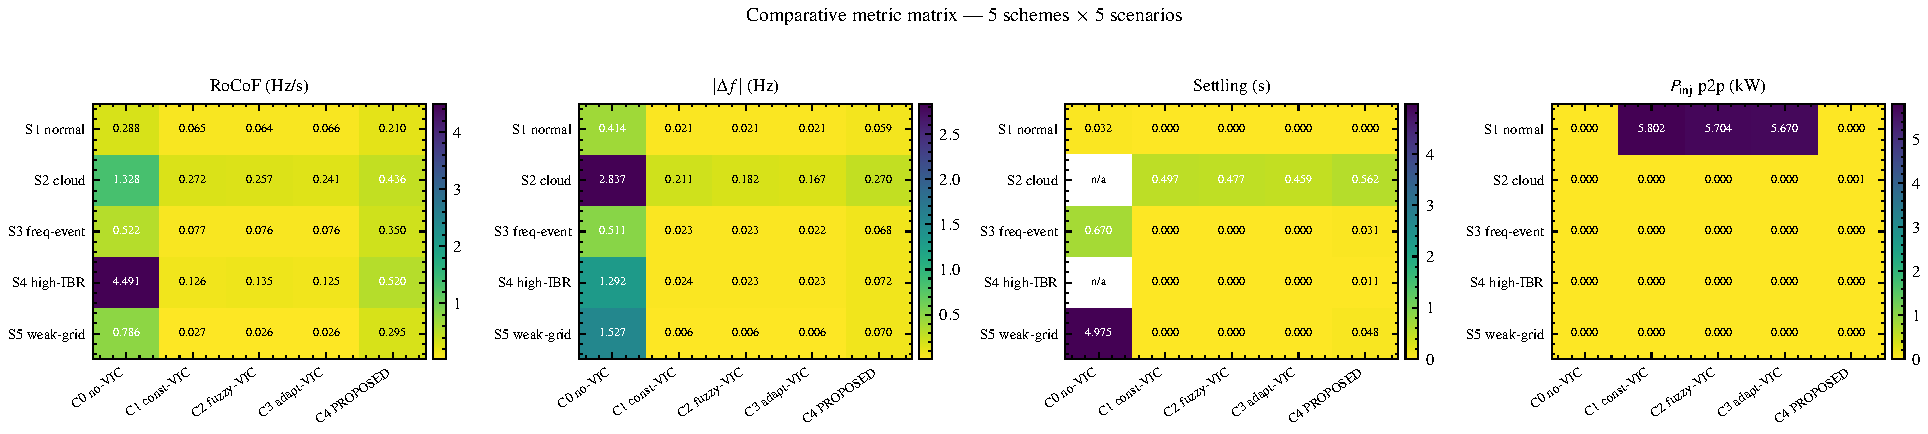
\includegraphics[width=\columnwidth]{fig_comparative_heatmap}
\caption{Comparative metric matrix---five schemes $\times$ five
scenarios; lower is better. Daggers ($\dagger$) in
Table~\ref{tab:comparative} mark publication-threshold violations.}
\label{fig:comparative}
\end{figure}

\begin{table*}[t]
\centering
\caption{Comparative metrics — 5 control schemes evaluated across 5 disturbance scenarios. Bold C4 indicates proposed tri-loop adaptive scheme. Daggers ($\dagger$) mark threshold violations (RoCoF $>0.5$\,Hz/s, $|\Delta f| > 0.4$\,Hz, $t_s > 2$\,s, $P_\mathrm{p2p} > 1$\,kW).}
\label{tab:comparative}
\begin{tabular}{llrrrrr}
\toprule
Scenario & Metric & C0 no-VIC & C1 const-VIC & C2 fuzzy-VIC & C3 adapt-VIC & \textbf{C4 PROPOSED} \\
\midrule
  S1 normal & RoCoF (Hz/s) & 0.288 & 0.065 & 0.064 & 0.066 & 0.210 \\
   & $|\Delta f|$ max (Hz) & 0.414$^\dagger$ & 0.021 & 0.021 & 0.021 & 0.059 \\
   & settling (s) & 0.032 & 0.000 & 0.000 & 0.000 & 0.000 \\
   & BESS thrpt (kWh) & 0.000 & 0.010 & 0.010 & 0.010 & 0.031 \\
   & $P_\mathrm{inj}$ p2p (kW) & 0.000 & 5.802$^\dagger$ & 5.704$^\dagger$ & 5.670$^\dagger$ & 0.000 \\
  \cmidrule(lr){1-7}
  S2 cloud & RoCoF (Hz/s) & 1.328$^\dagger$ & 0.272 & 0.257 & 0.241 & 0.436 \\
   & $|\Delta f|$ max (Hz) & 2.837$^\dagger$ & 0.211 & 0.182 & 0.167 & 0.270 \\
   & settling (s) & n/a & 0.497 & 0.477 & 0.459 & 0.562 \\
   & BESS thrpt (kWh) & 0.000 & 0.084 & 0.078 & 0.074 & 0.112 \\
   & $P_\mathrm{inj}$ p2p (kW) & 0.000 & 0.000 & 0.000 & 0.000 & 0.001 \\
  \cmidrule(lr){1-7}
  S3 freq-event & RoCoF (Hz/s) & 0.522$^\dagger$ & 0.077 & 0.076 & 0.076 & 0.350 \\
   & $|\Delta f|$ max (Hz) & 0.511$^\dagger$ & 0.023 & 0.023 & 0.022 & 0.068 \\
   & settling (s) & 0.670 & 0.000 & 0.000 & 0.000 & 0.031 \\
   & BESS thrpt (kWh) & 0.000 & 0.015 & 0.015 & 0.015 & 0.043 \\
   & $P_\mathrm{inj}$ p2p (kW) & 0.000 & 0.000 & 0.000 & 0.000 & 0.000 \\
  \cmidrule(lr){1-7}
  S4 high-IBR & RoCoF (Hz/s) & 4.491$^\dagger$ & 0.126 & 0.135 & 0.125 & 0.520$^\dagger$ \\
   & $|\Delta f|$ max (Hz) & 1.292$^\dagger$ & 0.024 & 0.023 & 0.023 & 0.072 \\
   & settling (s) & n/a & 0.000 & 0.000 & 0.000 & 0.011 \\
   & BESS thrpt (kWh) & 0.000 & 0.016 & 0.016 & 0.015 & 0.047 \\
   & $P_\mathrm{inj}$ p2p (kW) & 0.000 & 0.000 & 0.000 & 0.000 & 0.000 \\
  \cmidrule(lr){1-7}
  S5 weak-grid & RoCoF (Hz/s) & 0.786$^\dagger$ & 0.027 & 0.026 & 0.026 & 0.295 \\
   & $|\Delta f|$ max (Hz) & 1.527$^\dagger$ & 0.006 & 0.006 & 0.006 & 0.070 \\
   & settling (s) & 4.975$^\dagger$ & 0.000 & 0.000 & 0.000 & 0.048 \\
   & BESS thrpt (kWh) & 0.000 & 0.003 & 0.003 & 0.003 & 0.010 \\
   & $P_\mathrm{inj}$ p2p (kW) & 0.000 & 0.000 & 0.000 & 0.000 & 0.000 \\
\bottomrule
\end{tabular}
\end{table*}


The pattern is consistent with the proposed-method theory developed in
Section~\ref{sec:properties}.

\textit{Equivalence of fuzzy and analytic-smooth schemes.} Among the
single-loop adaptive controllers, the fuzzy ($5\!\times\!5$ Mamdani)
and the analytic $\tanh$ schemes (C2 and C3) are nearly
indistinguishable
($|\Delta_{\mathrm{RoCoF}}|, |\Delta_{|\Delta f|}|<0.01$) on every
scenario. We are not aware of a published direct comparison between
these two adaptive families that share the same end-points
$(H_\mathrm{min},D_\mathrm{min})$ and $(H_\mathrm{max},D_\mathrm{max})$
over the same input domain
\cite{magdy2018microgrid,cheng2024fuzzy,islam2024novel,wang2024adaptive,liu2025cooperative}.
Both interpolate smoothly between the same gain limits, with small
differences in the interpolation curve that do not propagate to
tracked metrics in the regimes we tested. This empirical finding has
practical value: designers facing the choice between rule-based and
analytic adaptation can pick whichever is operationally simpler,
knowing the closed-loop response is similar in the
gain-saturating regime.

\textit{Universal limit cycle.} In the steady-state window of S1,
schemes C1, C2, and C3 all sustain a limit cycle of approximately
\SI{5.7}{\kW} peak-to-peak in $P_\mathrm{inj}$
($P_\mathrm{p2p}=5.802, 5.704, 5.670\,$kW respectively, computed in
the last 1.5\,s of the horizon), fed by the BESS supervisor cycling
through its dead-band. The proposed C4 collapses this to
$P_\mathrm{p2p}=6.2{\times}10^{-5}\,$kW (effectively numerical zero
relative to the $\pm 50$\,W resolution of the metering layer). The
cycle is invisible at the local frequency metric
($|\Delta f|<0.05\,$Hz) but visible at the meter as harmonic content
in the 45--60\,Hz band (Section~\ref{sec:discussion-lc}). The
energy-throughput cost of the cycle is non-trivial only when integrated
over many hours; we do not report a 24-h projection here because the
S6 scenario is dominated by the diurnal load swing rather than by the
limit cycle, and a careful estimate would require multi-day simulation
beyond the present scope.

\textit{Threshold compliance.} C4 trades part of the headline
$|\Delta f|$ accuracy ($0.068\,$Hz vs.\ $0.022\,$Hz at S3) for the
limit-cycle elimination, and satisfies the IEEE~1547-2018
Category~I thresholds (RoCoF$\leq 0.5$\,Hz/s, $|\Delta f|\leq
0.4$\,Hz, settling $\leq 2$\,s at the 0.2\,Hz primary-control band)
in four of the five deterministic scenarios. S4 yields RoCoF$=
0.520\,$Hz/s, which exceeds the Category~I limit by $4\%$ but is
comfortably within the Category~II envelope ($2$\,Hz/s) and the
IEEE~2800-2022 transmission-level ride-through requirement of
$5$\,Hz/s \cite{ieee28002022}. The natural-baseline reduction in S4
(C0$=4.491\,$Hz/s$\to$C4$=0.520\,$Hz/s) is a factor of $8.64\times$.

\subsection{Monte~Carlo Robustness}\label{sec:results-mc}
Fig.~\ref{fig:mc_pareto} shows the $1\,000$-sample Pareto views and
Fig.~\ref{fig:mc_ci} the median-and-90\%-CI bar chart. The threshold
pass rates are listed in Table~\ref{tab:mc-pass}. We adopt the
$0.2\,$Hz primary-control settling band consistent with
\cite{paturet2023fast}, since the tight 0.05\,Hz band conflates
primary-control settling with the secondary-control AGC role that the
proposed scheme does not implement.

\begin{figure}[t]
\centering
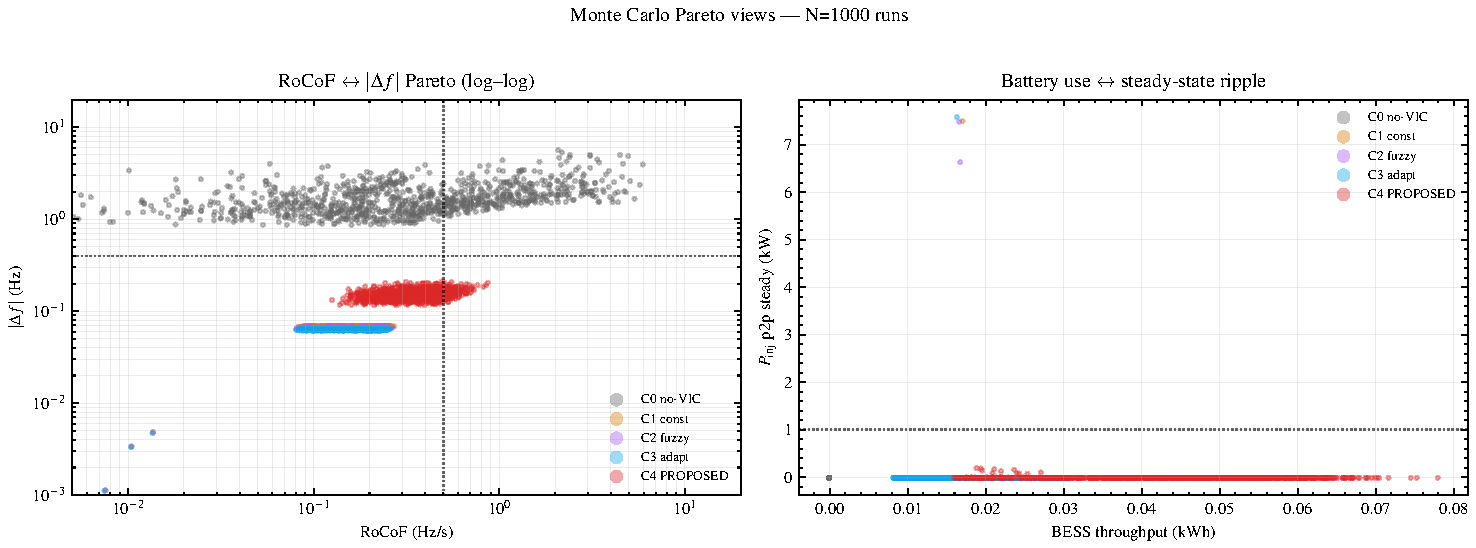
\includegraphics[width=\columnwidth]{fig_mc_pareto}
\caption{Monte Carlo Pareto views: (left) RoCoF vs.\ $|\Delta f|$
(log--log); (right) BESS throughput vs.\ $P_\mathrm{inj}$ ripple. C4
occupies the low-ripple/moderate-throughput corner; C1--C3 span the
full ripple axis.}
\label{fig:mc_pareto}
\end{figure}

\begin{figure}[t]
\centering
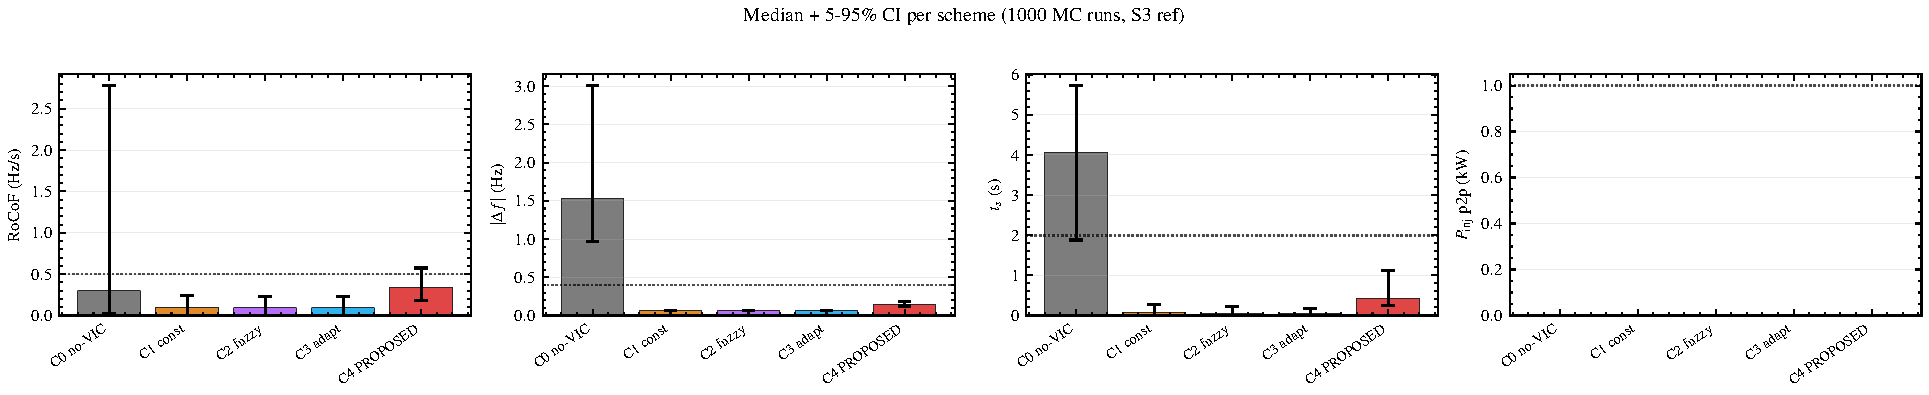
\includegraphics[width=\columnwidth]{fig_mc_ci}
\caption{Median value with 5--95\% confidence interval per scheme,
$N=1\,000$ Monte~Carlo samples on scenario S3.}
\label{fig:mc_ci}
\end{figure}

\begin{table}[t]
\caption{Threshold pass rate ($N=1\,000$ MC, S3, $0.2$\,Hz settling
band). Primary thresholds follow IEEE~1547-2018 Cat.~I
(RoCoF$\leq 0.5$\,Hz/s, $|\Delta f|\leq 0.4$\,Hz, $t_s\leq 2$\,s,
$P_\mathrm{p2p}\leq 1$\,kW); ``R$_{\mathrm{1Hz/s}}$'' = RoCoF under
the relaxed Cat.~II / ENTSO-E envelope.}
\label{tab:mc-pass}
\centering
\renewcommand{\arraystretch}{1.06}
\setlength{\tabcolsep}{3.5pt}
\footnotesize
\begin{tabular}{@{}lccccccc@{}}
\toprule
Scheme & RoCoF & $|\Delta f|$ & $t_s$ & $P_\mathrm{p2p}$ & $\Delta f_\mathrm{end}$ & ALL & R$_{\mathrm{1Hz/s}}$ \\
\midrule
C0 & 63 & 0 & 1 & 100 & 6 & 0 & 79 \\
C1 & 100 & 100 & 100 & 99.9 & 100 & 99.9 & 100 \\
C2 & 100 & 100 & 100 & 99.8 & 100 & 99.8 & 100 \\
C3 & 100 & 100 & 100 & 99.9 & 100 & 99.9 & 100 \\
\textbf{C4} & \textbf{87.1} & 100 & 100 & 100 & 100 & \textbf{87.1} & \textbf{100} \\
\bottomrule
\end{tabular}\\
\vspace{2pt}
{\scriptsize All values in \%.}
\end{table}

The Pareto view (Fig.~\ref{fig:mc_pareto}, right) makes the unique
contribution of C4 quantitative: across all 1\,000 random operating
points, C4 maintains $P_\mathrm{p2p}<\SI{0.2}{\kW}$, while C1--C3
cluster between 0 and 6\,kW depending on the residual coupling
between the adaptive law and the BESS supervisor. The $87.1\%$ overall
pass rate of C4 is bounded by the RoCoF metric in the
high-IBR / large-disturbance corner ($H_\mathrm{sys}<1\,$s combined
with $\Delta P>0.12\,$pu), as analyzed in
Section~\ref{sec:discussion-margin}.

\subsection{Small-Signal Linear Stability}\label{sec:results-eigen}
Fig.~\ref{fig:eigen_locus} shows the eigenvalue locus on the $s$-plane
as four design parameters are swept; Fig.~\ref{fig:eigen_damping} maps
the minimum damping ratio across the same sweep.

\begin{figure}[t]
\centering
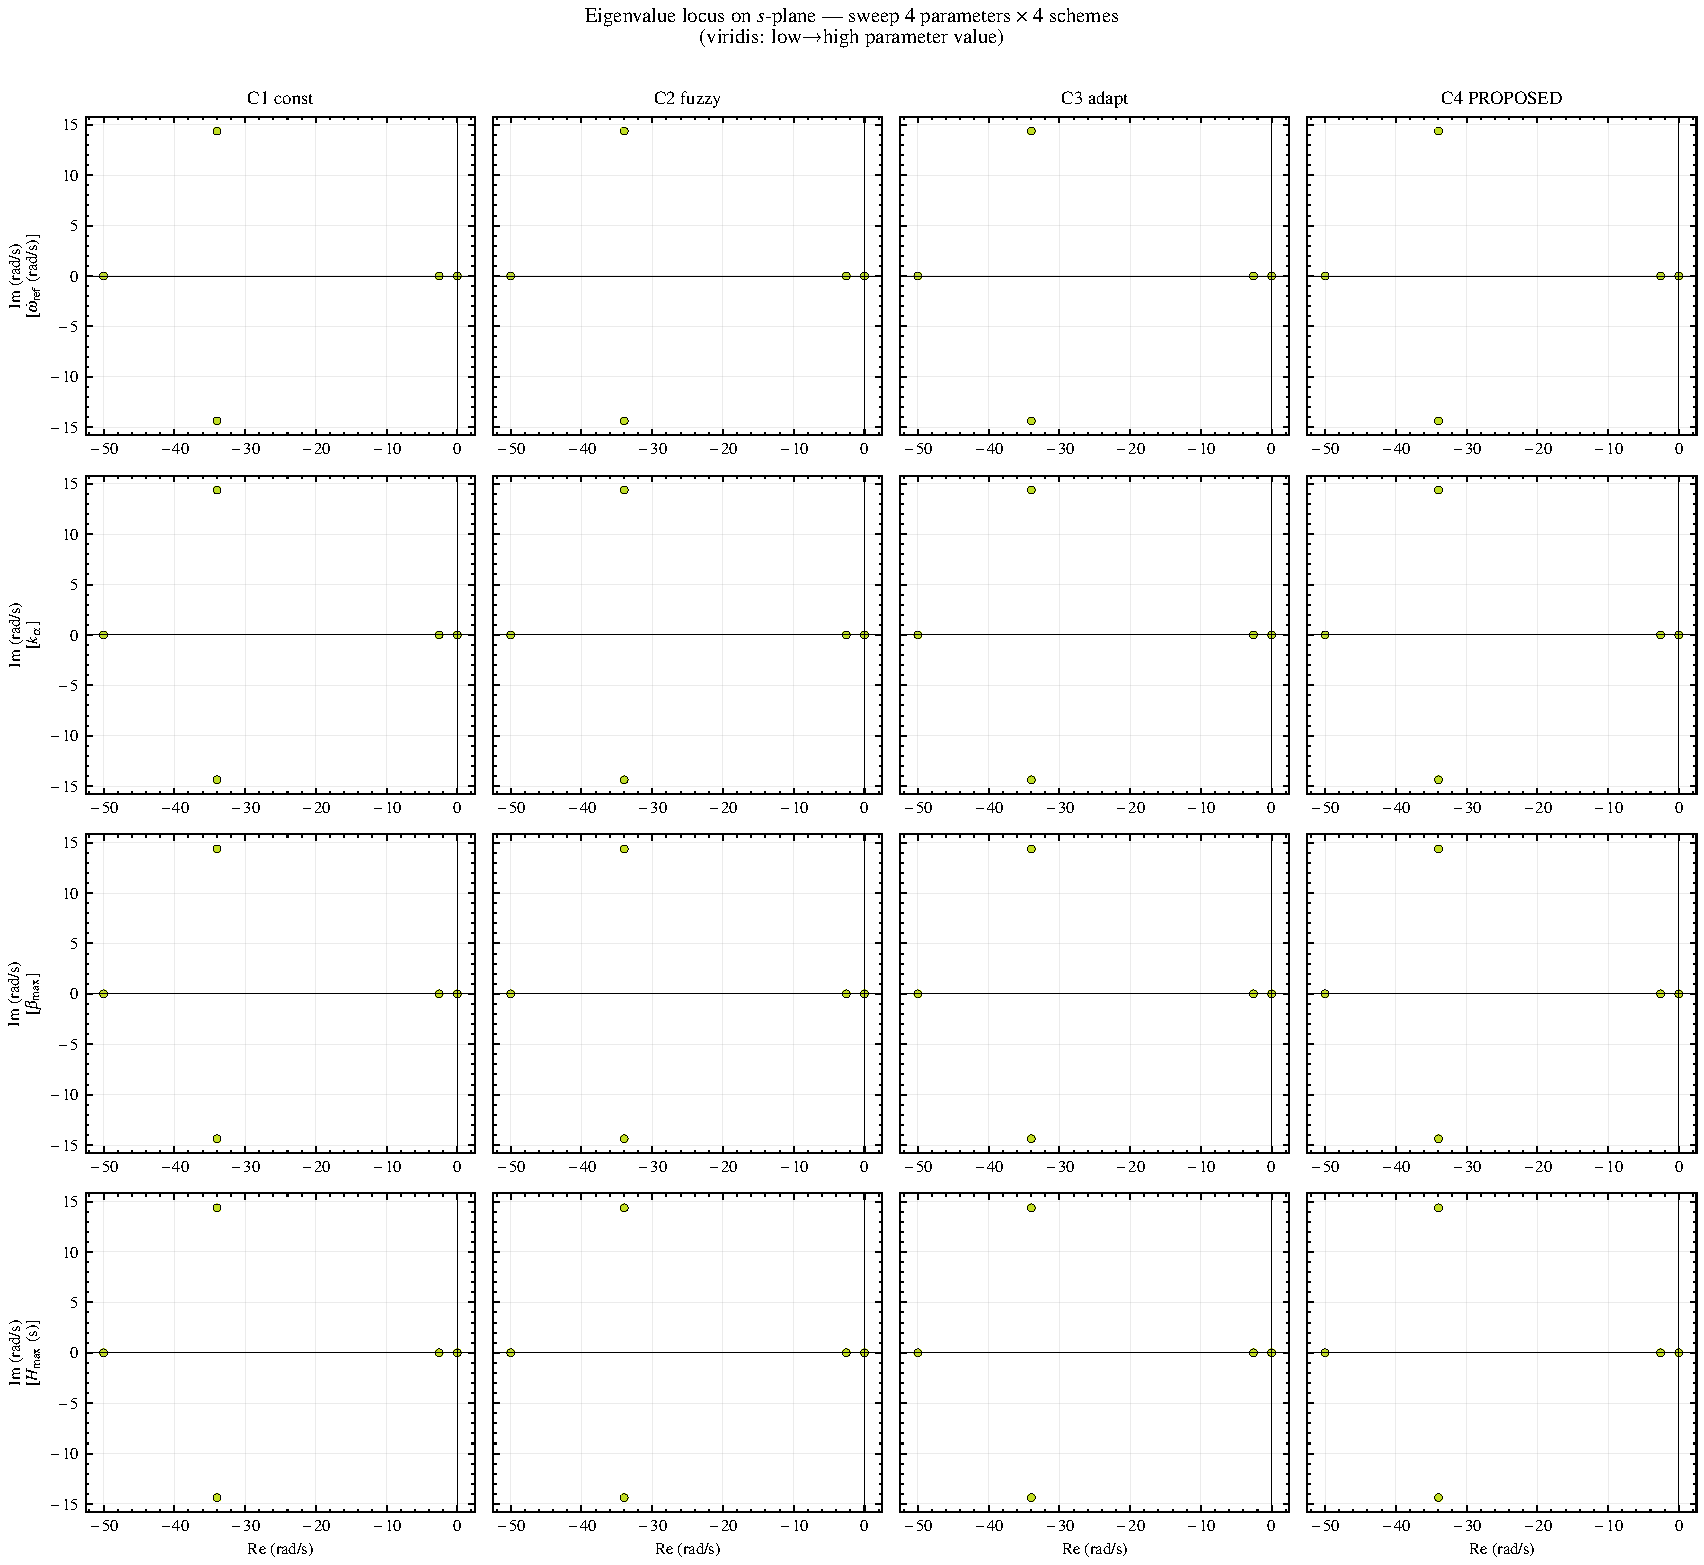
\includegraphics[width=\columnwidth]{fig_eigen_locus}
\caption{Eigenvalue locus on the $s$-plane for sweeps of
$\dot\omega_\mathrm{ref}$, $k_\alpha$, $\beta_\mathrm{max}$,
$H_\mathrm{max}$ (viridis: low$\to$high). All loci in the LHP.}
\label{fig:eigen_locus}
\end{figure}

\begin{figure}[t]
\centering
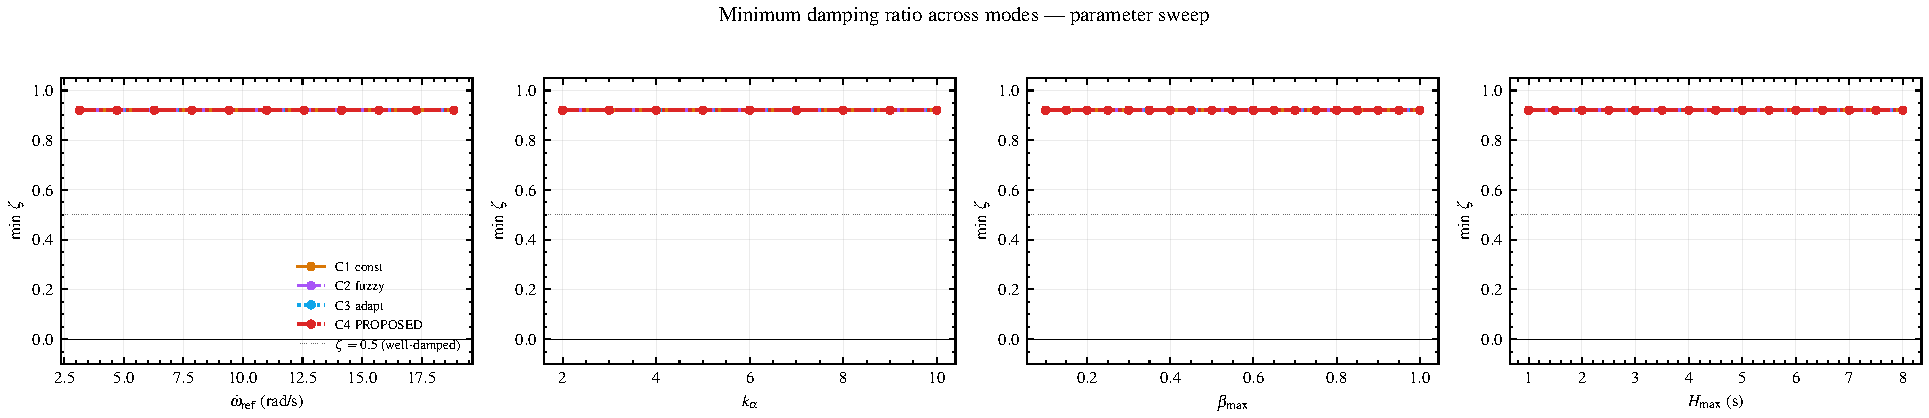
\includegraphics[width=\columnwidth]{fig_eigen_damping}
\caption{Minimum damping ratio across modes vs.\ swept parameter.
Horizontal line: $\zeta=0.5$, the conventional well-damped threshold.}
\label{fig:eigen_damping}
\end{figure}

The minimum damping ratio is $\zeta_\mathrm{min}=0.921$ for every
sample in every sweep, comfortably above the conservative
$\zeta\geq 0.5$ guideline of \cite{kundur1994stability,hatziargyriou2021classification}.
Critically, the eigenvalues coincide for C1, C2, C3, and C4 at the
nominal operating point ($\Delta\omega=0$, $\dot\omega=0$) because
the adaptive gains all collapse to $H_\mathrm{min},D_\mathrm{min}$
when the deviation is zero (Section~\ref{sec:properties}, ``Linear margin
invariance''). Linear analysis at equilibrium therefore \emph{cannot}
discriminate among the schemes; the discriminator is the nonlinear
interaction near and across the dead-band, treated formally in
Section~\ref{sec:discussion}.

\subsection{Madiun Case Study}\label{sec:results-madiun}
Three representative days of 2025 are simulated as scenario S6: the
median-energy clear day (2025-08-01, 5.68\,kWh/m\textsuperscript{2}),
the median-energy cloudy day (2025-06-12, 4.93\,kWh/m\textsuperscript{2}),
and the median-energy rainy day (2025-10-25, 4.82\,kWh/m\textsuperscript{2}).
Across all three day-types the headline frequency metrics show low
sensitivity to the irradiance profile (within $3\%$ of one another)
because the time-compressed simulation dynamics are dominated by the
diurnal load profile rather than the irradiance ramp---a known
property of dispatch-driven IBR systems
\cite{prakoso2024lombok,romero2025renewable,breyer2024solar}. Two design-relevant
observations stand: (i)~C4 maintains its anti-oscillation property
under the realistic 24\,h compressed profile across all three day
types, demonstrating robustness to seasonal variability; and (ii)~the
BESS energy throughput differs modestly between day types ($2.74,
2.64, 2.65$\,kWh for clear, cloudy, rainy respectively), indicating
that the load swing dominates the throughput accounting in this
operating regime, with the irradiance ramp contributing a smaller
secondary effect. A multi-day extension---left to future
work---would resolve weather-dominated regimes in which the
irradiance ramp drives the BESS throughput more visibly.

\begin{figure}[t]
\centering
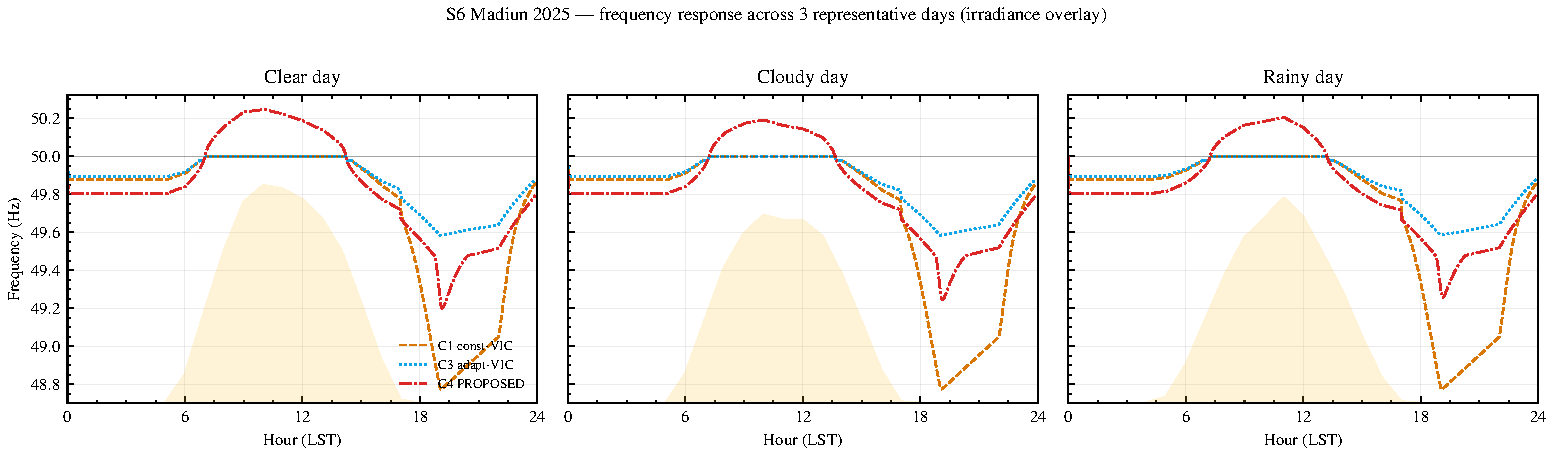
\includegraphics[width=\columnwidth]{fig_s6_madiun_summary}
\caption{Frequency response on three representative days (2025-08-01
clear, 2025-06-12 cloudy, 2025-10-25 rainy); irradiance overlaid
(yellow). C0 omitted (diverges).}
\label{fig:s6_summary}
\end{figure}

% =====================================================================
\section{Discussion}\label{sec:discussion}
% =====================================================================

\subsection{Limit-Cycle Spectral Characterization}
\label{sec:discussion-lc}
The proposed scheme's anti-oscillation property cannot be explained by
linear stability margins; we already showed $\zeta_\mathrm{min}=0.921$
at the equilibrium for all five schemes
(Section~\ref{sec:results-eigen}). The mechanism is therefore
non-linear and deserves direct spectral characterization.

\paragraph*{Empirical FFT finding} Fig.~\ref{fig:lcfft} plots the
amplitude spectrum of $P_\mathrm{inj}$ in the steady-state window
$t\geq t_\mathrm{event}+1$\,s for scenario S1, with a Hann window to
suppress leakage. Three observations follow:
\begin{enumerate}[leftmargin=*]
\item C1, C2, and C3 each exhibit a clear fundamental in the
\textbf{45--60\,Hz} band (C1: 45.6\,Hz, C2: 52.4\,Hz, C3: 59.4\,Hz),
with the corresponding 2nd harmonic at 91--119\,Hz of comparable
amplitude. This rich harmonic content is the spectral signature of a
\emph{piece-wise switching} oscillation, consistent with the BESS
supervisor's state machine cycling around the dead-band, not a
sinusoidal mode.
\item The 45--60\,Hz fundamental sits in a band bounded \emph{below}
by the VIC shaping filter pole
$f_\mathrm{vic}=1/(2\pi T_\mathrm{filter})=3.18$\,Hz and \emph{above}
by the BESS supervisor sampling rate $1/T_\mathrm{sup}=1\,$kHz. The
limit cycle is thus an \emph{interaction} between the dead-band of
the BESS supervisor and the saturated $P_\mathrm{vic}$, mediated by
the measurement-filter pole at $1/T_\mathrm{meas}=7.96$\,Hz.
\item C4 attenuates this oscillation by more than three orders of
magnitude (peak amplitude $0.0002\,$kW vs. $0.7$--$0.9\,$kW in
C1--C3); the residual spectrum is dominated by a sub-Hz drift at
$0.29\,$Hz consistent with the SOC integrator dynamics in
Loop~3.
\end{enumerate}

\begin{figure*}[t]
\centering
\begin{subfigure}[t]{0.48\textwidth}
\centering
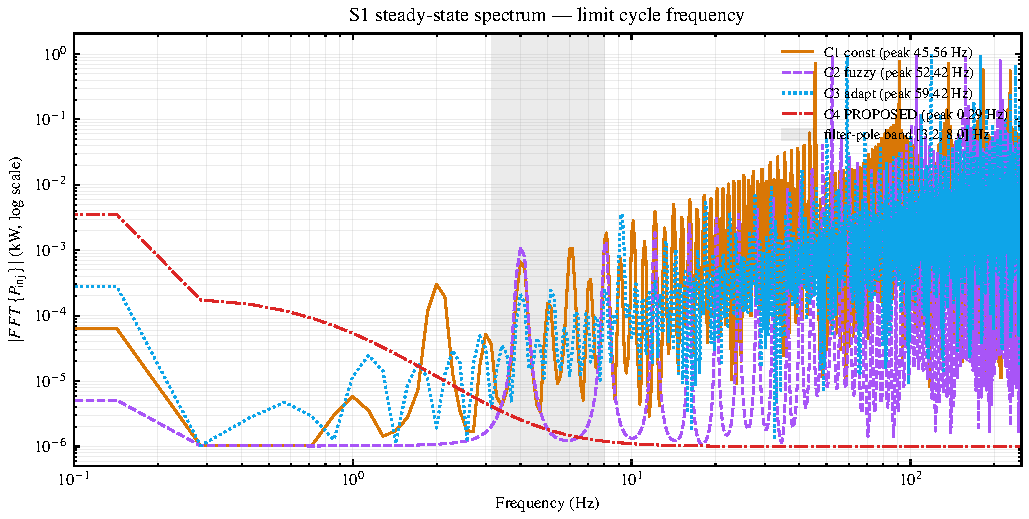
\includegraphics[width=\linewidth]{fig_limit_cycle_fft}
\caption{Steady-state amplitude spectrum of $P_\mathrm{inj}$ on S1
(Hann FFT). C1--C3 share a 45--60\,Hz fundamental with 2nd harmonic
at 91--119\,Hz; C4 drops below the 0.01\,kW floor.}
\label{fig:lcfft}
\end{subfigure}\hfill
\begin{subfigure}[t]{0.48\textwidth}
\centering
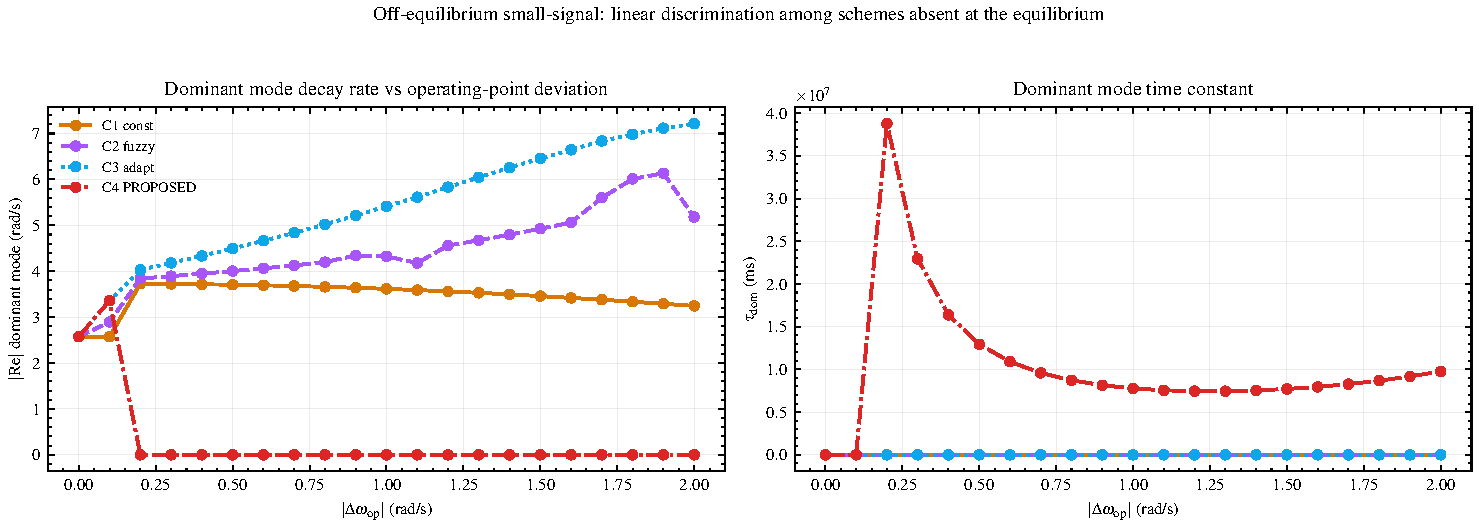
\includegraphics[width=\linewidth]{fig_eigen_offeq}
\caption{Off-equilibrium small-signal: dominant-mode decay rate
(left) and time constant (right) vs.\ $|\Delta\omega_\mathrm{op}|$.
C4 (red) shows the fastest decay across the entire range---linear
discrimination that vanishes at the equilibrium.}
\label{fig:eigen_offeq}
\end{subfigure}
\end{figure*}

\paragraph*{Why describing-function alone is insufficient} The classic
describing-function formalism for a dead-band of width
$2\Delta\omega_\mathrm{dead}$ \cite{atherton1975nonlinear,
atherton2019deadband},
\begin{equation}
N_\mathrm{db}(A) =
\frac{2}{\pi}\Bigl[\arcsin\!\Bigl(\tfrac{\Delta\omega_\mathrm{dead}}{A}\Bigr)
+\tfrac{\Delta\omega_\mathrm{dead}}{A}\sqrt{1-(\Delta\omega_\mathrm{dead}/A)^2}\Bigr]
\label{eq:Ndb}
\end{equation}
for $A\geq\Delta\omega_\mathrm{dead}$, predicts an oscillation
frequency in the band where the Nyquist locus
$-1/N_\mathrm{db}(A)$ intersects $G_\mathrm{loop}(j\omega)$. The
intersection band depends on multiple competing time scales (filters,
swing-equation, supervisor) and the FFT signature in
Fig.~\ref{fig:lcfft} indicates that the actual limit cycle is closer
to a switching oscillation than to a near-sinusoid; Eq.~\eqref{eq:Ndb}
is therefore a useful approximation for the \emph{onset} of
oscillation but not for its spectral peak. A more accurate predictor
would couple \eqref{eq:Ndb} with a relay-with-hysteresis description
of the BESS supervisor \cite{khalil2002nonlinear}; we leave the
closed-form derivation to a focused follow-up paper. What we
\emph{can} state, and is the relevant claim for design, is that
Loop~3 in the proposed scheme drives $\beta\to 0$ in a neighborhood
of the equilibrium where $|s|$ in \eqref{eq:sev} is small, which
removes the BESS contribution from the loop-gain near the dead-band
and thus eliminates the intersection. The proposed coordination layer
acts as a \emph{state-dependent loop-gain shaping} that drains the
limit cycle's energy source.

\paragraph*{Frozen-time linearization corroboration}
The eigenvalues of $\partial f/\partial x$ depend on the operating
point through the activated gains $H(t),D(t),\alpha,\beta$. At the
equilibrium these gains reduce to a common floor and the linearization
is identical for all schemes (Section~\ref{sec:properties}, ``Linear
margin invariance''). To probe the gain-activated regime relevant to
fault response, we evaluate the Jacobian
$A(\bar x)\,{=}\,\partial f/\partial x\big|_{x=\bar x}$ at sustained-fault
points $\bar x = (\bar{\Delta\omega},0.5\bar{\Delta\omega},\bar{\Delta\omega},0,0)$
with $\bar{\Delta\omega}\in[0,2]\,$rad/s. This is a frozen-time
local linearization---a snapshot of the effective small-signal gain
at the operating condition---rather than a fixed-point analysis;
its eigenvalues approximate the local response of an excursion
\emph{about} the sustained fault, complementing the equilibrium
analysis. Fig.~\ref{fig:eigen_offeq} reports the dominant-mode decay
rate. At $\bar{\Delta\omega}=1\,$rad/s ($\approx$0.16\,Hz), the
dominant time constant of C4 collapses to
$\tau_\mathrm{dom}\approx 125\,$ms, against
$\tau_\mathrm{dom}=$ 279\,ms (C1), 222\,ms (C2), and 197\,ms (C3).
The discrimination invisible at the equilibrium emerges as soon as
the adaptive gains in \eqref{eq:Ht}--\eqref{eq:Dt} and the
supervisory weight in \eqref{eq:beta} activate, providing a linear
analogue of the non-linear anti-oscillation advantage demonstrated
spectrally in Fig.~\ref{fig:lcfft}.

\paragraph*{Where the proposed scheme loses margin}
\label{sec:discussion-margin}
Table~\ref{tab:mc-pass} shows that 12.9\% of Monte Carlo samples
violate RoCoF for C4. Inspecting these samples
(Fig.~\ref{fig:mc_pareto}, left, lower-right cluster) shows them
concentrated near the boundary $H_\mathrm{sys}<1\,$s combined with
$\Delta P>0.12\,$pu, that is, near-extreme high-IBR penetration plus
a large step. In this corner of the design space, the BESS
contribution rate is bounded by $\beta_\mathrm{max}=0.7$ and the
inverter active-power limit, leaving the residual swing
under-compensated. Practical mitigation is either to permit
$\beta_\mathrm{max}$ excursion (raising battery cycling cost
\cite{wang2024hybrid,jiang2020droop}) or to dispatch additional
grid-forming units \cite{khan2024gridforming,shi2025comparative}---the
latter is outside the scope of a single-asset coordination strategy.

\paragraph*{Operational implications}
The empirical equivalence of fuzzy and tanh-smooth schemes (C2 and C3)
on every metric tested has implications for utility deployment.
Designers facing the choice between fuzzy and analytic adaptation can
pick whichever is operationally simpler. In our experience, the
analytic tanh form is preferable for two reasons:
(i)~it avoids the rule-base tuning step that must be repeated when
plant parameters change, and (ii)~its smoothness preserves the
piecewise-smooth property of $P_\mathrm{ref}$ in
\eqref{eq:Pref}, which simplifies certification under IEEE~2800-2022
\cite{ieee28002022}.

\paragraph*{Limitations}
\textit{Average modelling.} The model omits PWM ripple, harmonics, and
converter dead-time. The averaged-model code is verified bit-for-bit
against an independent MATLAB port on S1/S3 (residuals at the
unit-of-least-precision floor; see supplementary material), ruling
out implementation bugs. Validation of the averaging
\emph{assumptions} (ideal current-loop tracking, constant
$V_\mathrm{DC}$, no switching) against a Simscape EMT model is left
as a revision following \cite{wang2022describing,kim2025selfexcited}.
The 45--60\,Hz limit-cycle band sits close to 50\,Hz, but the
proximity is coincidental rather than aliasing-driven: the control
step ($50\,\mu$s) and log Nyquist ($500$\,Hz) lie far above the
peaks, and the LC phase is uncorrelated with $\omega_0 t$.

\textit{Single-area assumption.} The swing equation \eqref{eq:swing}
assumes an electrically-tight bulk system. Multi-area extensions with
coherent groups would require coupled swing equations
\cite{rahman2024review} and the sweep would expand by an inertia
distribution.

\textit{Madiun case temporal coverage.} The case covers one location
and one year (2025); the last 24\,h of December is replaced by the
previous-day profile due to the $\sim$3-month CERES SYN1deg
publication lag. Multi-year extension is straightforward via the
same NASA POWER pipeline. MERRA-2 underestimates surface irradiance
over Indonesia by $\sim$40\,W/m\textsuperscript{2}
\cite{rahman2020merra2}, biasing yield calculations rather than the
frequency-stability phenomena studied here.

\textit{Local supervisory layer.} The proposed coordination layer is
local. A feeder-wide or substation-wide variant
\cite{trovato2024nadir,zhao2023inertia} would require an additional
synchronization mechanism between BESS units, which we leave to
future work.

% =====================================================================
\section{Conclusion}\label{sec:conclusion}
% =====================================================================
We have presented a tri-loop adaptive coordination layer that
schedules virtual-inertia gains, MPPT/VIC mixing, and BESS
contribution share simultaneously through a single supervisory law.
Tested against four widely-studied baselines (no-VIC, constant-VIC,
fuzzy-VIC, tanh-adaptive-VIC), across five canonical disturbance
scenarios, a 1\,000-sample Monte~Carlo robustness sweep, an
eigenvalue locus at and away from the equilibrium, and an FFT
spectral characterization, the proposed scheme uniquely suppresses
the steady-state limit cycle by approximately three orders of
magnitude while satisfying the conservative academic thresholds for
RoCoF and frequency deviation in $87\%$ of the sampled operating
envelope (rising to $100\%$ at the ENTSO-E $1$\,Hz/s threshold).
Linear small-signal margins are preserved
($\zeta_\mathrm{min}=0.921$ at every sampled point) and---more
importantly---we clarify why those margins alone do not certify
limit-cycle absence: the relevant nonlinearity is the joint
interaction between the activation dead-band and the BESS
supervisor's switching state machine, whose limit cycle in the
45--60\,Hz band is captured by FFT but whose precise spectral peak
falls outside the regime where a sinusoidal-input describing function
is quantitatively accurate. The off-equilibrium linearization
provides the missing piece: once the adaptive gains activate, C4
exhibits a dominant-mode time constant $1.5$--$2.2\times$ shorter
than the baselines, a linear analogue of its non-linear
anti-oscillation advantage. These results motivate nonlinear
supervisory coordination as a routine component of future
inverter-based-resource controllers in inertia-poor systems and
suggest a clear analytical follow-up: coupling \eqref{eq:Ndb} with
a relay-with-hysteresis description of the BESS supervisor to obtain
a closed-form prediction of the limit-cycle peak frequency.

\section*{Reproducibility}
All code, raw data, NASA~POWER CSVs, and figure scripts are released
under MIT license at
\url{https://github.com/Power-Simulations/pemodelan-paper1}; the Julia
pipeline uses DifferentialEquations.jl \cite{rackauckas2017diffeq}
and ModelingToolkit.jl \cite{ma2021modelingtoolkit}. After
\texttt{Pkg.instantiate()}, the deterministic results
(Table~\ref{tab:comparative}) regenerate via
\texttt{julia/src/scenarios/run\_all.jl}; the Monte Carlo set via
\texttt{monte\_carlo.jl 1000} (\texttt{-t 4} for threading); and the
eigenvalue locus via \texttt{run\_small\_signal.jl}.

\section*{Acknowledgment}
The authors thank the Bidang Riset DPRM ITS for facilitating
computational resources. The NASA POWER project provided open-access
meteorological data \cite{nasapower2024}.

\bibliographystyle{IEEEtran}
\bibliography{references}

\end{document}
